\documentclass[11pt]{article}

\usepackage[margin=1.1in]{geometry}
\usepackage[T1]{fontenc}
\usepackage[utf8]{inputenc}
\usepackage{lmodern}
\usepackage{microtype}
\usepackage{graphicx}
\usepackage{booktabs}
\usepackage{amsmath}
\usepackage[numbers,sort&compress]{natbib}
\usepackage{xcolor}
\usepackage[colorlinks=true,linkcolor=blue!60!black,citecolor=blue!60!black,urlcolor=blue!60!black]{hyperref}
\usepackage{caption}
\usepackage{multicol}
\captionsetup{font=small,labelfont=bf}

% let tall figures actually place near their references instead of drifting to the end
\renewcommand{\topfraction}{0.92}
\renewcommand{\textfraction}{0.06}
\renewcommand{\floatpagefraction}{0.75}

\newcommand{\eg}{e.g.,\ }
\newcommand{\ie}{i.e.,\ }

\title{\textbf{The One-Word Census: Answer-Choice Conformity Across 44 Language Models}}
\author{Tapan Parikh\\Cornell Tech\\\texttt{tsp53@cornell.edu}}
\date{July 2026}

\begin{document}
\maketitle

\begin{abstract}
\noindent
When a language model must choose one answer from a large space of equally valid options, which answer does it choose --- and how often is it the same answer every other model chooses? Asked to ``pick a word --- any word,'' 44 language models spanning five years of releases and more than a dozen labs chose \emph{serendipity} 41\% of the time. We characterize this convergence, and each model's degree of participation in it, with a deliberately minimal instrument: 31 single-turn prompts, each naming a category with a wide space of valid one-word answers (``Name a tree.''), asked four times to each model with no system prompt. Because the datum is a discrete choice, analysis is exact-match on normalized tokens --- no embeddings, no judge --- and the whole battery costs roughly a dollar per model. That models converge is by now well documented; our contribution is the instrument, and what it reveals about the structure of the convergence. We score each model by \emph{answer-choice surprisal}: the average $-\log_2$ probability of its answers under the pooled answers of all other models, leave-one-out. The field's convergence is extreme --- in 7 of 31 categories a single answer accounts for over 80\% of all answers across the panel --- but conformity varies more than fourfold in answer likelihood across models, and the variation is structured. Lightly post-trained and persona-tuned models are the most divergent; the newest mainline flagships are the most conformist, producing almost no answer that no other model produced. Within four lineages (Claude, GPT, Qwen, Grok), conformity increases steadily with generation. However, the trend reverses for the latest flagship Claude and GPT models --- a possible early signal of repositioning at the top tier. Rankings are robust to roster composition (leave-one-family-out $\rho = 0.985$). Strikingly, divergence itself is convergent: models that avoid the modal answer overwhelmingly land on the \emph{same} runner-up (\eg \emph{mustard} takes 95\% of non-\emph{ketchup} condiment answers), and after conditioning on a one-dimensional ``depth'' propensity, no significant pairwise affinity between any two models survives ($0$ of $946$ pairs). Against human category-production norms, the field is more concentrated than people in 18 of 20 shared categories (its modal answer takes 66\% of answers vs.\ 36\% of human first responses). All prompts, transcripts, and code are public.
\end{abstract}

\section{Introduction}
\label{sec:intro}

A common complaint about conversational AI is that its answers feel generic --- as if they came off a shelf. This paper measures one concrete, quantifiable form of that genericity: when a language model must choose one answer from a large space of equally valid options, which answer does it choose, and how often is that the same answer every other model chooses?

The experimental object is deliberately simple. We ask ``Name a tree. Reply with one word only.'' There are hundreds of familiar trees; any of them is correct. A population of independent reasoners --- or a single reasoner sampling at temperature 1.0 --- could spread its probability mass widely. What we observe instead is near-total collapse: across 44 models from more than a dozen labs, \emph{oak} accounts for 94\% of all answers. Tools: \emph{hammer}, 94\%. Flowers: \emph{rose}, 91\%. Vegetables: \emph{carrot}, 90\%. And with no category constraint at all (``Pick a word.''), the single most common answer --- \emph{serendipity} --- takes 41\% of a pool drawn from the entire English lexicon.

That models converge is by now well documented \citep{wenger2025different,jiang2025hivemind,zhang2025noveltybench}. Our contribution is not the phenomenon but an instrument for it, and what the instrument reveals about its structure:

\begin{enumerate}
\item \textbf{A cheap, mechanical, per-model conformity score.} We define \emph{answer-choice surprisal} (\S\ref{sec:metric}): a leave-one-out measure of how unlikely a model's answers are under the pooled answers of the rest of the field. It requires no embeddings, no LLM judge, and no human annotation; the full battery is ${\sim}120$ API calls (roughly \$1) per model.
\item \textbf{A scorecard of 44 models with structured variation} (\S\ref{sec:scorecard}). Conformity spans $1.05$ to $3.21$ bits. The most divergent models are lightly post-trained, persona-tuned, or retrieval-grounded; the most conformist are the newest mainline flagships, several of which produce essentially zero answers that no other model gave.
\item \textbf{Generational trajectories} (\S\ref{sec:generations}). Within the Claude, GPT, Qwen, and Grok lineages, later releases are more generally conformist. However, the trend reverses for the latest flagship Claude and GPT models.
\item \textbf{Robustness} (\S\ref{sec:robustness}, \S\ref{sec:pairwise}). Rankings survive leave-one-family-out scoring and roster resampling, and a three-level test for pairwise affinity between models comes up empty.
\item \textbf{The runner-up consensus} (\S\ref{sec:pairwise}). Even when models leave the modal answer, they overwhelmingly land on the \emph{same} runner-up (\eg \emph{mustard} takes 95\% of non-\emph{ketchup} condiment answers). Even the divergence is convergent.
\item \textbf{Calibration against a human population} (\S\ref{sec:human}). Against human category-production norms from cognitive psychology, the field is more concentrated than people in 18 of 20 shared categories (its modal answer takes 66\% of the field vs.\ 36\% of human first responses).
\end{enumerate}

\section{Related work}
\label{sec:related}

\paragraph{The finding: models converge.}
\citet{jiang2025hivemind} document mode collapse on 26K real open-ended queries at two levels --- intra-model repetition and, even stronger, inter-model homogeneity --- and show that LLM judges and reward models systematically prefer the modal outputs. \citet{wenger2025different} find that on standard creativity tests, model outputs are far more similar to each other than human responses are, regardless of vendor. \citet{zhang2025noveltybench} benchmark distributional diversity directly and find models produce significantly less distinct-and-high-quality variation than human writers --- with larger models within a family often \emph{less} diverse than smaller siblings, an inversion our generational results echo behaviorally. \citet{wright2025epistemic} measure diversity at the level of factual claims across 155 topics and find every one of 27 models less epistemically diverse than a plain web search. \citet{gueorguieva2026templatic} find six models share a single discourse-level empathy template covering 83--90\% of their emotional-support responses. \citet{santurkar2023whose} show model opinion distributions cluster on a particular demographic slice; the CAIS values dashboard \citep{cais2025values} finds models rank the world nearly identically in forced-choice preference elicitation. Whatever level one measures --- token, answer, claim, discourse move, worldview --- the field converges.

Relative to this literature, our instrument trades breadth for three properties the prior work lacks: it is \emph{mechanical} (exact-match; recomputable from transcripts with no model in the loop), \emph{cheap enough to run at every release}, and \emph{per-model} --- it produces a scorecard, not just a population-level statement. The intra/inter distinction of \citet{jiang2025hivemind} maps onto our separation of self-consistency from conformity (\S\ref{sec:metric}).

\paragraph{The mechanism: post-training collapses the mode.}
\citet{kirk2024rlhf} establish the canonical trade-off: RLHF improves out-of-distribution generalisation but significantly reduces output diversity. \citet{gxchen2025kl} show that common KL-regularized RLHF settings specify \emph{unimodal} target distributions --- the objective is non-diverse by construction. \citet{zhang2024diffuse} show instruction-tuned models cannot be random on request (Mistral picks the name ``Avery'' at $40\times$ its population rate) and that the fix is training-side, not prompt-side. \citet{liu2026alignmenttax} localize within-model homogenization to preference-optimization stages via base-vs-instruct ablations (1\% vs.\ 28.5\% single-semantic-cluster rates); \citet{karouzos2026where} trace where in post-training lineages diversity is lost. The earliest articulation of the phenomenon in RLHF-tuned models is \citet{janus2022mode}; the generic-response problem itself predates LLMs entirely \citep{li2016diversity}. We treat mechanism as background: our measurements are black-box and cannot localize causes (\S\ref{sec:limitations}), but the mechanism literature makes the behavioral patterns we find --- conformity concentrated in the most heavily post-trained models --- unsurprising in direction, if not in magnitude.

\paragraph{The stakes: convergence propagates.}
Humans who create with these models are individually lifted and collectively flattened: GPT-4-assisted stories are better \emph{and} more alike \citep{doshi2024generative}; LLM-assisted ideation homogenizes without users noticing \citep{anderson2024homogenization}; the effect traces specifically to the aligned model \citep{padmakumar2024writing}. Meanwhile models train on a web increasingly written by models, and recursive training destroys distributional tails first \citep{shumailov2024curse,guo2024curious}. \citet{wright2025epistemic} name the plausible end state \emph{knowledge collapse}. On the correction side, diversity-aware post-training now exists \citep{li2025darling}; if it lands in production systems, a fixed public instrument run on every release is what would detect the turn.

\paragraph{Methodology.}
Diversity metrics disagree because ``diversity'' conflates form and content \citep{tevet2021evaluating} --- our exact-match answer-choice design is a response to exactly this (\S\ref{sec:whyoneword}). Single-sample evaluation misleads and providers do not reliably honor sampling parameters \citep{song2024greedy} --- hence four samples per cell and separate reporting of conformity and self-consistency. \citet{chen2023chatgpt} demonstrated that fixed prompt sets detect behavioral drift within months --- then the measurement stopped; the eval-transparency and conversation-dump traditions \citep{liang2023helm,zheng2024lmsys,zhao2024wildchat} publish transcripts but not a fixed instrument over time, while the preservation problem is argued \citep{johnson2024deprecating} and answered so far only first-party \citep{anthropic2025deprecation}.

\section{The instrument}
\label{sec:method}

\subsection{Stimulus}
\label{sec:stimulus}

The stimulus is 31 single-turn prompts, frozen before data collection. Thirty are category prompts of the form \emph{``Name a[n] $X$. Reply with one word only.''} where $X$ is a category with a wide space of valid one-word answers: color, animal, fruit, vegetable, city, country, flower, sport, musical instrument, bird, gemstone, tree, beverage, insect, occupation, language, dessert, tool, fish, metal, fabric, herb, dance, hobby, condiment, cheese, dinosaur, mythical creature, board game, and emotion. The thirty-first removes the category constraint entirely: \emph{``Pick a word. Reply with one word only.''} There is no system prompt; each prompt is a fresh single-turn conversation; \texttt{max\_tokens} is 1024 and requested temperature is 1.0 for every model.

\subsection{Answer-choice surprisal}
\label{sec:metric}

For model $m$ and category $c$, let $A_{m,c}$ be $m$'s answers (up to four samples) and let the \emph{field} be the multiset of all other models' answers to $c$: $F_{-m,c} = \biguplus_{o \neq m} A_{o,c}$. Each answer $a \in A_{m,c}$ is scored by its add-one-smoothed leave-one-out surprisal,
\begin{equation}
s(a) \;=\; -\log_2 \frac{\mathrm{count}_{F_{-m,c}}(a) + 1}{\,|F_{-m,c}| + V_c\,},
\qquad V_c = \bigl|\,\mathrm{support}(F_{-m,c}) \cup \mathrm{support}(A_{m,c})\,\bigr|,
\end{equation}
and a model's headline score is the mean of $s(a)$ over all its valid answers across all categories (informally: the \emph{Mustard Quotient}). The score is measured in bits: each additional bit means the model's answers are, on average, half as likely under the rest of the field. A model that always gives the field's answer scores near the theoretical floor; a model that reaches for \emph{gouda} where the field says \emph{cheddar} scores higher. Smoothing ensures a never-seen answer is informative rather than infinitely surprising.

Three companion statistics separate ways of being different:
\begin{itemize}
\item \textbf{modal avoidance} --- the fraction of a model's answers that differ from the field's single most common answer for that category;
\item \textbf{novel rate} --- the fraction of answers that \emph{no} other model ever gave (the strongest tell of genuine divergence);
\item \textbf{self-distinctness} --- distinct answers divided by samples, within model and category (within-model spread).
\end{itemize}
Surprisal and self-distinctness measure different things --- a model can be original and steady (stable off-modal defaults) or merely noisy (high sampling spread). Self-distinctness is deliberately reported rather than corrected away: requested temperature is not honored uniformly across providers \citep{song2024greedy}, so within-model spread doubles as a measured proxy for effective sampling temperature (\S\ref{sec:limitations}).

\subsection{Normalization and data hygiene}
\label{sec:normalization}

Replies are normalized to a single token: lowercased, stripped of punctuation and emoji, and reduced to the final alphabetic word --- which correctly handles models that ignore the one-word instruction (``A common color is blue.'' $\rightarrow$ \emph{blue}). A mechanical junk guard treats the following as \emph{failed cells} rather than answers: chat-template artifacts (\eg \texttt{[/INST]}, markup tags), replies longer than 15 words (truncated chain-of-thought would otherwise contribute a spurious ``novel'' final word), bare acknowledgments (``Okay.''), and single-letter tokens. Within each category pool, bare plurals are merged with their singulars when both occur. Of $44 \times 31 \times 4 = 5456$ attempted cells, 5439 (99.7\%) yield a valid answer. The final-word rule does not manufacture novelty: only 13 of those valid cells contain more than one word, and in all but one the extracted token is the answer a reader would take from the reply.

Uncertainty on each model's headline score is a bootstrap 90\% confidence interval (2000 draws) that resamples categories and pools per-answer surprisals, matching the answer-weighted estimand of the headline mean.

\subsection{Why one-word answers and exact match}
\label{sec:whyoneword}

The design principle is that the datum is the \emph{discrete choice}, not the phrasing. The one-word clamp is identical for every model, so it cannot differentiate them, and it makes the metric verbosity-immune by construction. This avoids the form/content conflation \citet{tevet2021evaluating} warn about, and exact match on normalized tokens is the cure. The cost is scope: the instrument measures \emph{choice character}, not tone, style, or discourse structure (\S\ref{sec:limitations}).

\subsection{Panel}
\label{sec:panel}

The panel is 44 models served via OpenRouter, which routes each call to a hosting provider --- the model's own lab for the closed frontier models, or one of several third-party hosts for open weights --- spanning US frontier labs across multiple generations (GPT-3.5 through GPT-5.6, including all three tiers of the same-day GPT-5.6 release; Claude 3 through Claude 5; Gemini 2.5--3.5; Grok 4.20 through 4.5), Chinese labs (DeepSeek, Qwen, GLM, Kimi, Hunyuan, Ernie), enterprise and search-tuned models (Command~A, Palmyra, Granite, Sonar), persona- and community-tuned models (Hermes~4, WizardLM-2, MythoMax), and small open models (Mixtral, Llama, Gemma). Each model was queried four times per prompt in July 2026. The full model list with metadata is frozen in the repository.

\section{Results}
\label{sec:results}

\subsection{The substrate: a strong mode almost everywhere}
\label{sec:substrate}

\begin{figure}[tp]
\centering
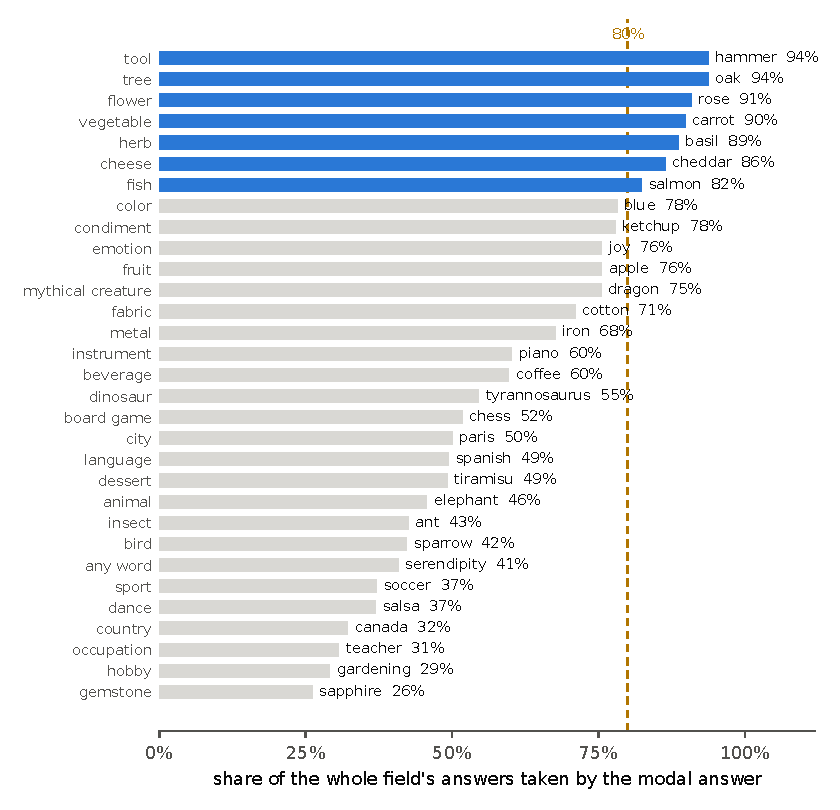
\includegraphics[width=0.98\linewidth]{figs/substrate.pdf}
\caption{Modal-answer share by category, pooled over all 44 models ($\sim$176 answers per category). Blue bars mark categories where a single answer takes ${\geq}80\%$ of the entire field's answers. Direct labels give the modal answer.}
\label{fig:substrate}
\end{figure}

Figure~\ref{fig:substrate} shows the pooled answer distribution's concentration for each category. In 7 of 31 categories, a single answer accounts for at least 80\% of every answer given by every model: \emph{hammer} (94\%), \emph{oak} (94\%), \emph{rose} (91\%), \emph{carrot} (90\%), \emph{basil} (89\%), \emph{cheddar} (86\%), \emph{salmon} (82\%); \emph{ketchup} (78\%), \emph{blue} (78\%), and \emph{apple} (76\%) sit just below the line. At the diffuse end are exactly the categories with no single prototypical exemplar in text: gemstone (26\%), hobby (29\%), occupation (31\%), country (32\%), dance (37\%), sport (37\%).

The unconstrained prompt is the conceptually sharpest case. Given the entire English lexicon, the field still collapses: \emph{serendipity} takes 71 of 174 answers (41\%), followed distantly by \emph{apple} (16), \emph{ephemeral} (7), and \emph{sunshine} (6) --- 52 distinct words in total from a possible space of hundreds of thousands. Every constrained category at least has the excuse of a salient exemplar; here there was no constraint at all.

\paragraph{The mode is the frictionless answer, not the frequent one.}
Reading the full pooled distributions shows the modal answer is not the most common referent in the world, nor the most discussed: it is the blandest \emph{unambiguous} exemplar. Two clean cases. Fruit: \emph{apple} 133, \emph{mango} 35, \emph{banana} 7, \emph{orange} 1 --- orange, among the most common fruits in life and text, is a singleton, plausibly because it collides with the color. Vegetable: \emph{carrot} 158, \emph{broccoli} 15, \emph{tomato} 0 --- across 176 answers the single most-discussed ``is it a vegetable?'' item in English never appears.\footnote{That case is confounded: \emph{tomato} is botanically a fruit, so a model may simply be right to omit it. \emph{Orange} above carries the point without the confound --- an unambiguous, common fruit that all but vanishes for no reason but a color collision.} Similarly, in a panel dominated by US-lab models, the United States is named exactly once in 174 country answers (\emph{USA}, by one model, once); the field's mode is \emph{canada} 56, \emph{japan} 41, \emph{france} 41. Answers with an edge --- a homonym collision, a taxonomic argument, a possible connotation --- are systematically absent.

\subsection{The scorecard: conformity varies widely, and the variation is structured}
\label{sec:scorecard}

\begin{figure}[tp]
\centering
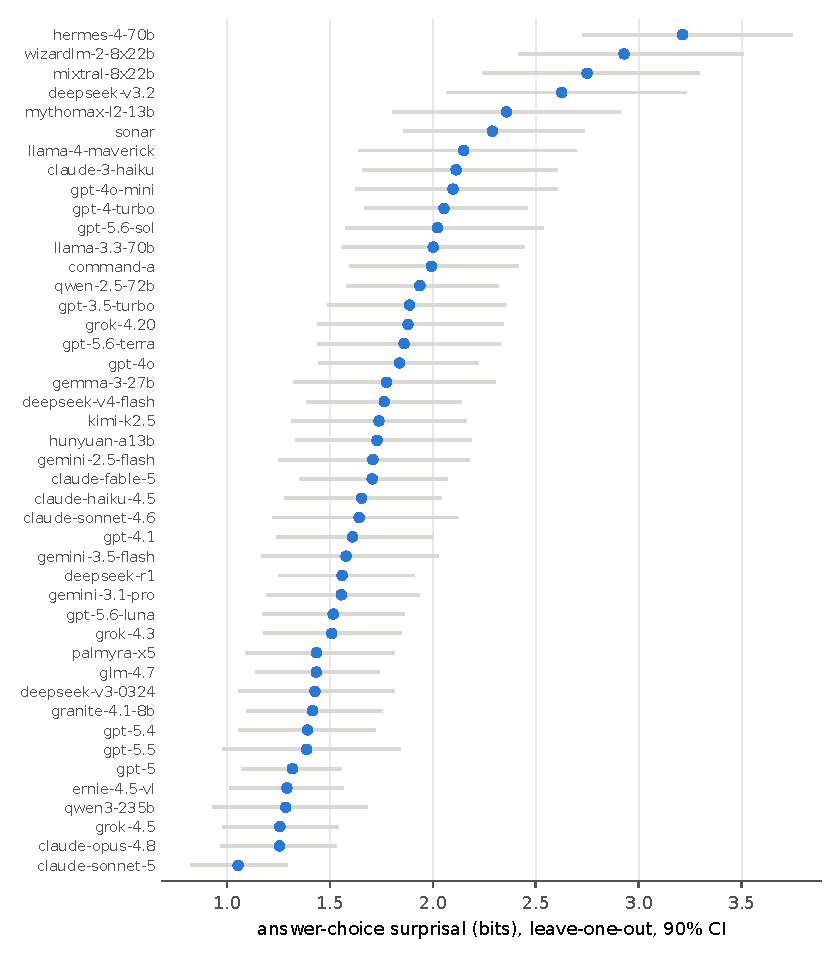
\includegraphics[width=0.9\linewidth]{figs/scorecard.pdf}
\caption{Answer-choice surprisal for all 44 models (bits; leave-one-out against the pooled field; add-one smoothed), with bootstrap 90\% CIs from resampling categories. Higher = answers the field does not give.}
\label{fig:scorecard}
\end{figure}

Figure~\ref{fig:scorecard} and Table~\ref{tab:scorecard} (appendix) give the full scorecard. The range is wide --- 1.05 to 3.21 bits, a factor of more than four in answer likelihood under the field.

\paragraph{The divergent tail is lightly post-trained.}
The top of the scorecard is dominated by persona- and community-tuned models: Hermes~4~70B (3.21 bits; 21\% of its answers novel to the field; 58\% modal avoidance), WizardLM-2 (2.93), Mixtral 8x22B (2.75), MythoMax (2.36). Grouping by panel origin, the persona/community group averages 2.83 bits against 1.72 for US frontier models, 1.68 for Chinese-lab models, and 1.61 for enterprise models. The one search-grounded model, Sonar (2.29), is a further singular case consistent with a different objective producing different defaults: retrieval grounding pulls answers off the parametric consensus. This divergence is not disguised incapacity: the divergent leaders' answers are unimpeachable category members that are simply not the crowd's pick --- \emph{crocodile}, \emph{camembert}, \emph{verdigris} where the field gives \emph{elephant}, \emph{cheddar}, \emph{blue}.

\paragraph{The conformist tail is the newest flagships.}
The bottom five are Claude Sonnet~5 (1.05), Claude Opus~4.8 (1.25), Grok~4.5 (1.26), Ernie 4.5 (1.29), and Qwen3 235B (1.29) --- with GPT-5 (1.32) and GPT-5.4/5.5 (both 1.39) close by. These are, essentially without exception, the newest, most heavily post-trained mainline assistants in the panel, and they produce almost nothing the rest of the field does not produce: Sonnet~5, Opus~4.8, Ernie, and GPT-5 all have novel rates of 0\%. Sonnet~5 avoids the modal answer on only 19\% of its answers.

\paragraph{Within-lab dissociations.}
Claude Fable~5 --- released by the same lab in the same month and generation as Claude Sonnet~5 --- scores 1.71 against Sonnet~5's 1.05. Its divergence comes not from sampling spread (self-distinctness 0.32, among the lowest) but from stable, repeatable, off-modal defaults --- \emph{gouda} for cheese, \emph{mustard} for condiment, \emph{mango} for fruit, four runs out of four. It essentially never produces a field-novel answer (its choices are drawn from the field's existing support); it simply does not default to the field's first choice. The $0.65$-bit separation is not a bootstrap artifact: a paired permutation over categories --- shuffling the two models' labels within each category, 10{,}000 draws --- rejects exchangeability at $p < 0.001$.\footnote{Per-answer surprisals are scored leave-one-out against the full 44-model field, so a permuted label shifts one model in or out of the reference pool --- a negligible, symmetric effect at this panel size. Script: \texttt{probe\_permutation.py}.}

The GPT-5.6 release replicates the dissociation at a second lab: its three tiers span Luna 1.52, Terra 1.86, Sol 2.02 (Sol vs.\ Luna: $0.51$ bits, paired permutation $p = 0.004$). Terra's divergence is Fable-shaped --- with some of the \emph{same} stable defaults (\emph{mustard} and \emph{mango}, four runs out of four) and self-distinctness (0.37) indistinguishable from its conformist siblings. 

Same-generation siblings from two labs occupying opposite ends of the mid-field demonstrate, purely behaviorally, that answer-choice conformity is not determined by lab, scale, or release date: it is set per-release. It is not, however, set at random: at both labs the \emph{amount} of divergence orders by tier, with the most divergent current model the largest, most expensive flagship (Sonnet~5 1.05 $<$ Opus~4.8 1.25 $<$ Fable~5 1.71; Luna 1.52 $<$ Terra 1.86 $<$ Sol 2.02). Read as a trend, this ordering may signal a repositioning at the premium tier --- the workhorse tiers converging on the interchangeable consensus answer while the flagship is allowed, or tuned, to stay off it. Our black-box measurements cannot localize the cause (training corpora, post-training, RLHF, etc.).

\subsection{Generational trajectories}
\label{sec:generations}
\begin{figure}[tp]
\centering
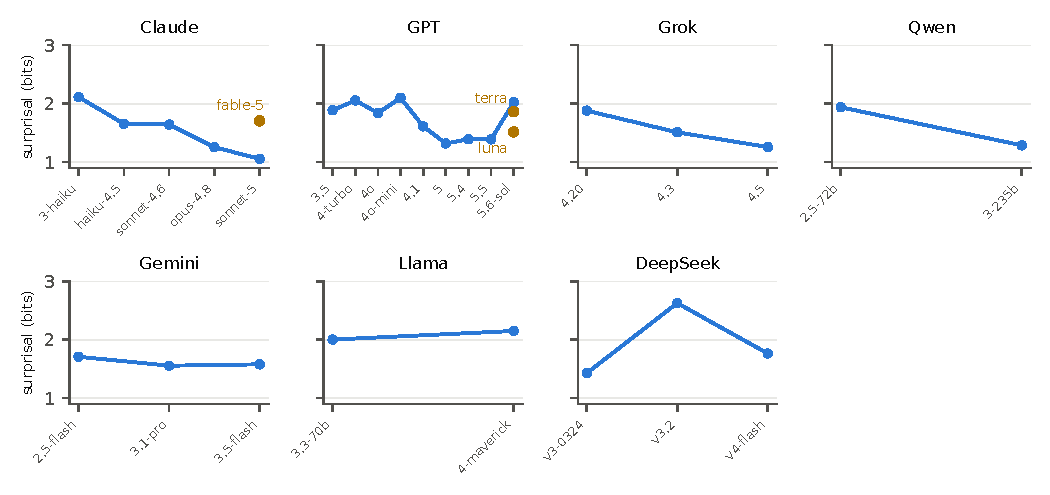
\includegraphics[width=0.98\linewidth]{figs/walks.pdf}
\caption{Answer-choice surprisal across release generations within seven families (shared $y$-axis). Claude, GPT, Qwen, and Grok all decline, until the latest releases from Anthropic and OpenAI; Gemini is flat; Llama rises; DeepSeek is non-monotonic. The blue walk traces each family's conformist mainline; amber points are the divergent premium siblings beside it --- Claude Fable~5 beside Sonnet~5, and the GPT-5.6 premium tiers Terra and Sol beside their smaller sibling Luna.}
\label{fig:walks}
\end{figure}

Figure~\ref{fig:walks} tracks surprisal across releases within seven families. Claude declines steadily along its mainline: 3-Haiku 2.11 $\rightarrow$ Haiku-4.5 1.65 $\rightarrow$ Sonnet-4.6 1.64 $\rightarrow$ Opus-4.8 1.25 $\rightarrow$ Sonnet-5 1.05 (last in the panel), with Fable~5 (1.71) the off-trend exception. Grok declines steepest of all: 4.20 1.88 $\rightarrow$ 4.3 1.51 $\rightarrow$ 4.5 1.26, from mid-field explorer to third-from-last in three releases. Qwen slides from 1.94 (2.5-72B) to 1.29 (Qwen3-235B). GPT peaks in its 4-era --- 3.5 1.89 $\rightarrow$ 4-turbo 2.05 $\rightarrow$ 4o 1.84 / 4o-mini 2.10 --- descends steeply through 4.1 (1.61) into the 5-era (5: 1.32; 5.4: 1.39; 5.5: 1.39), and then \emph{reverses} at 5.6, whose three same-day tiers order by tier: Luna 1.52, Terra 1.86, Sol 2.02 --- the flagship back at 4-era divergence. Against these, Gemini is flat (1.71 / 1.56 / 1.58), Llama \emph{rises} (2.00 $\rightarrow$ 2.15), and DeepSeek is non-monotonic (the v3.2 anomaly).

\emph{Newer = more conformist} is a pattern (Claude, GPT, Qwen, Grok), not a universal law --- and at both leading labs the newest flagship broke it in the week of measurement: GPT reverses at 5.6 after five straight declines, and Claude's Fable~5 stands off-trend above its mainline. Where the decline occurs it is steep --- and it is sharpest exactly where a strong mode exists: on the most concentrated categories (modal share ${\geq}80\%$), the newest mainline flagships (Sonnet~5, Opus~4.8, GPT-5, GPT-5.5, Qwen3) average 0.36 bits --- near the theoretical floor of always giving the field's modal answer --- against 1.07 bits for each family's oldest panel member; on the diffuse categories the same cohorts score 2.20 against 2.88. The newest flagships snap to the mode hardest exactly where the mode is strongest. The direction is consistent with the bigger-is-less-diverse finding of \citet{zhang2025noveltybench} and with the post-training mechanism literature (\S\ref{sec:related}), but our roster does not fully separate size from generation, and each model is measured at one date. The GPT-5.6 tier ordering (Luna $<$ Terra $<$ Sol) is itself an inversion of bigger-is-less-diverse \emph{within} a generation: the largest, most expensive tier is the most divergent --- and Anthropic's generation-5 pair repeats the ordering (Sonnet~5 $<$ Fable~5), the two labs' premium flagships diverging in the same measurement month (\S\ref{sec:scorecard}).

\paragraph{Divergence is a post-training property, not lineage DNA.}
The DeepSeek panel of Figure~\ref{fig:walks} is the caveat against reading these walks as family destiny. In that lineage, v3-0324 scores 1.43, v3.2 jumps to 2.63 (10\% novel; the panel's only frontier-lab explorer), v4-flash regresses to 1.76, and R1 sits at 1.56. The contrast between the two extremes is stark in the raw transcripts: at the same requested temperature, v3-0324 gives four-out-of-four \emph{identical} answers in 23 of 31 categories (\emph{lion}$\times$4, \emph{eagle}$\times$4, \emph{tokyo}$\times$4, \emph{hammer}$\times$4, \emph{dragon}$\times$4, \ldots), while v3.2 scatters into the deep tail (\emph{kiwi}, \emph{esperanto}, \emph{charleston}, \emph{stargazing}, \emph{crimson}); their answer sets differ in 23 of 31 categories.\footnote{Because routing floated in the main run, we re-ran a subset of categories with both models pinned to the \emph{same} host; the contrast reproduces in full (v3-0324 four-for-four on its defaults, v3.2 scattering), so it is not an artifact of which provider happened to serve each call. Probe script and transcripts are in the repository.}

What makes this pair unusually informative is that the lineage is a single continued-training chain: per DeepSeek's release documentation \citep{deepseek2025changelog}, v3-0324 is a post-training refresh of the same pretrained V3 base, and v3.2 descends from it through continued training and a new RL recipe --- there is no separate pretraining run anywhere in the chain. The gap between a bottom-tier conformist and the panel's only frontier-lab explorer is therefore attributable to post-base training choices, not to different pretraining corpora. Whatever made v3.2 divergent was specific to that release's recipe --- not persistent lab DNA, and not scale, recency, or origin.


\subsection{Robustness: the rankings are not a roster artifact}
\label{sec:robustness}

Because scoring is leave-one-out against the pooled panel, a fair objection is that the scorecard measures the roster: the panel-mean score is just the field's entropy, the fourfold typing is a median split of this panel, and a model from a well-represented family is scored partly against its own relatives. We concede what is true by construction --- absolute bit values are relative to this field --- and test what is not: whether the \emph{rankings} are roster artifacts. Three checks, using no new API calls:

\begin{itemize}
\item \textbf{Leave-one-family-out (LOFO).} Rescoring every model against a field with all its relatives removed yields Spearman $\rho = 0.985$ against the shipped ranking. Sibling contamination is real, small, and GPT-concentrated (gpt-5.6-sol gains $+0.24$ bits, moving rank $11\rightarrow 9$; the panel now carries eleven GPT models); no headline result moves --- Hermes is first and Sonnet~5 last either way.
\item \textbf{Balanced fields.} Scoring against one randomly drawn model per family (200 draws): the top three rank 1--3 in \emph{every} draw, the fourth ranks 4th or 5th, and Sonnet~5 ranks 44th in \emph{every} draw.
\item \textbf{Random subsets.} Against random 15-model fields (200 draws): top and bottom stable; mid-pack ranks wobble $\pm 3$--$5$.
\end{itemize}

The generational declines survive LOFO scoring unchanged. One residue cannot be tested away: the panel is an availability sample of what OpenRouter serves, not usage-weighted. But usage weighting would make the reference field \emph{more} flagship-dominated, sharpening the headline contrasts, so the sampling bias runs against our findings rather than for them. The substrate results (\S\ref{sec:substrate}) are pooled-distribution facts across $\sim$15 independent labs and are least exposed to the critique.

\subsection{No pairwise affinity --- and the runner-up consensus}
\label{sec:pairwise}

\begin{figure}[tp]
\centering
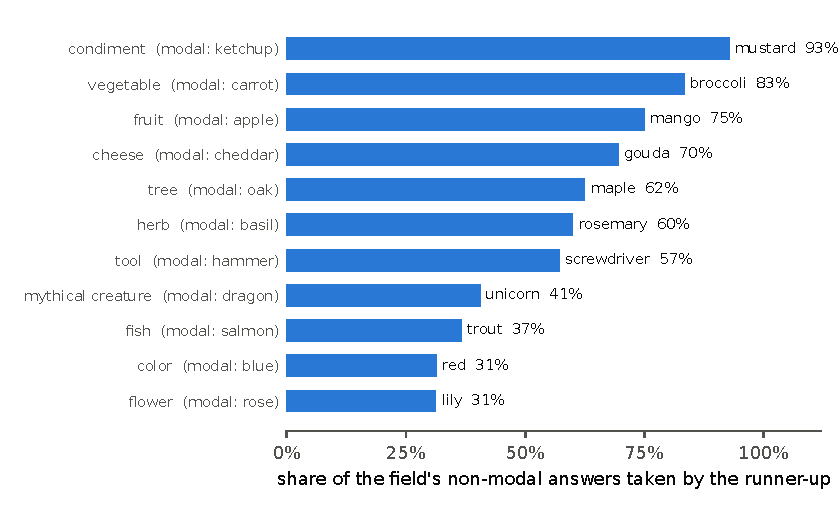
\includegraphics[width=0.95\linewidth]{figs/runnerup.pdf}
\caption{The runner-up consensus. For each high-concentration category (modal share ${\geq}75\%$), the share of the field's \emph{non-modal} answers taken by the single most common non-modal answer. When models deviate from the mode, they overwhelmingly deviate to the same place.}
\label{fig:runnerup}
\end{figure}

We tested for pairwise affinity across all $\binom{44}{2} = 946$ model pairs with a three-level ladder, each level conditioning away a population structure the previous level mistook for affinity (Benjamini--Hochberg FDR, $q = .05$; Monte Carlo nulls where normal approximations fail on small counts). Level 1 (rarity-weighted co-occurrence against a random-partner null) leaves five apparent pairs --- but is confounded by avoidance propensity: two habitual modal-avoiders will co-occur against a conformist null with no coupling at all. Level 2 (conditioning on avoidance) leaves eighteen --- tellingly, led by same-family pairs (gpt-5.6-luna $\times$ gpt-5.6-sol strongest, grok-4.20 $\times$ grok-4.3 second) --- but is confounded by a \emph{depth} propensity: how far down the field's answer distribution a model lands when off-modal is a stable per-model trait. Level 3, conditioning on both: \textbf{zero of 946 pairs survive.}

The null result is more interesting than the affinities it dissolves, because of what the conditioning variables turn out to be:

\begin{enumerate}
\item \textbf{The runner-up consensus} (Figure~\ref{fig:runnerup}). The off-modal distribution has its own mode, and it is nearly as concentrated as the primary one: \emph{mustard} takes 95\% of non-\emph{ketchup} condiment answers, \emph{broccoli} 83\% of non-\emph{carrot}, \emph{mango} 81\% of non-\emph{apple}, \emph{gouda} 71\% of non-\emph{cheddar}. Even when a model avoids the consensus, it avoids it in the consensus way.
\item \textbf{Depth propensity is one-dimensional.} Among each model's distinct off-modal answers, the fraction landing on the field's \#2--\#3 answers (rather than deeper) is a stable trait: Opus~4.8 100\%, Grok~4.5 94\%, Ernie 92\%, Sonnet~5 90\%, Fable~5 74\% (a ``runner-up club''), versus Hermes 35\%, MythoMax 38\%, DeepSeek v3.2 38\%, WizardLM-2 39\% (genuine deep-tail divers). Given a model's position on this single axis, its specific choices are statistically exchangeable with the field's.
\end{enumerate}

A caveat cuts both ways: 31 categories $\times$ 4 samples is low power for pairwise tests, so weak affinities would be invisible; by the same token, none of the level-1/level-2 ``hits'' should ever be quoted as findings. (That the level-2 survivors are led by same-family sibling pairs, and that even these dissolve under depth conditioning, is the ladder working as designed: family resemblance is real but fully mediated by the two propensities.)

\paragraph{Prompting reaches conditional modes, not the tail.}
Asking for divergence does not release the distribution; it opens a new column with its own mode. Prompted \emph{``Name an unusual fruit,''} the panel produced just 12 distinct fruits: \emph{durian} takes 44\%, \emph{rambutan} 34\%, and the top three answers take 84\% of the field. Conditioning on unusualness triples the distinct-answer count of the unconditioned fruit prompt (12 vs.\ 4) --- but the mass immediately re-concentrates on the prototypes of the new frame. This is consistent with the training-side findings of \citet{zhang2024diffuse}: the collapse lives in the weights, and prompting navigates between conditional modes rather than drawing from variance.

\subsection{Compared to a human population}
\label{sec:human}

\begin{figure}[tp]
\centering
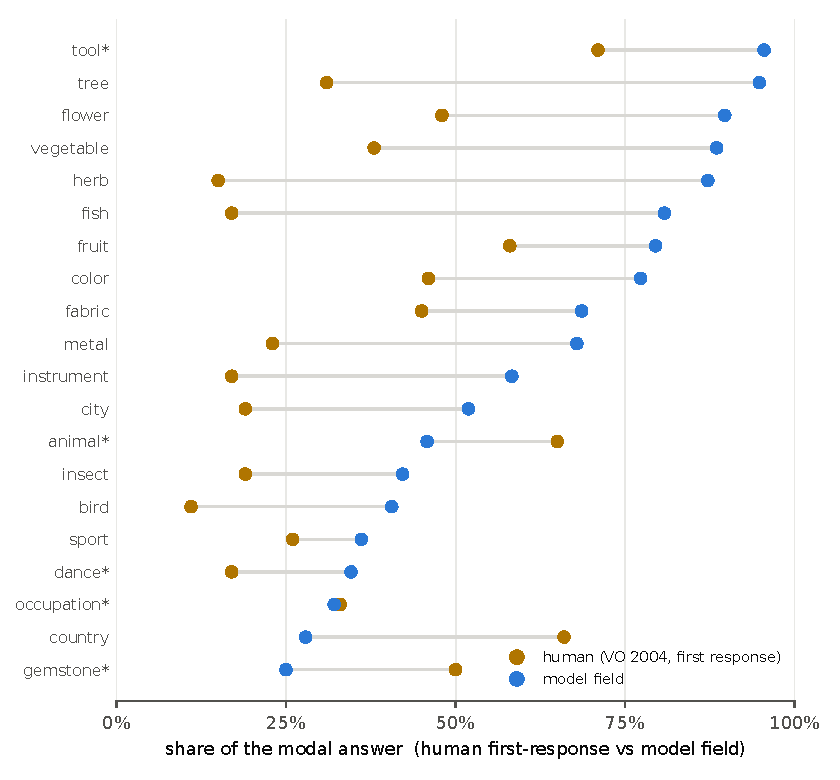
\includegraphics[width=0.82\linewidth]{figs/humannorms.pdf}
\caption{Concentration of the modal answer, model field vs.\ human population, on the 20 categories shared with the Van Overschelde norms. Human = the fraction of people who gave the answer as their \emph{first} response; model = modal share of the 44-model field (VO-exact wording for the six categories whose wording differs). The model field is more concentrated (blue right of amber) in 18 of 20; \emph{country} reverses, and \emph{occupation} by a hair.}
\label{fig:humannorms}
\end{figure}

How concentrated is the field \emph{relative to people}? The Battig--Montague category-production norms \citep{battig1969norms}, updated by \citet{vanoverschelde2004norms}, record for each exemplar the proportion of participants who produced it as their \emph{first} response --- a single-response human distribution for 20 of our categories. (For the six whose norm wording differs from ours --- ``a four-footed animal,'' ``a carpenter's tool,'' ``a precious stone,'' and three more --- we use the exact-wording rerun so the comparison is matched.)\footnote{The wording is important. Our census wording ``Name a gemstone'' produces the flattest mode in the battery --- \emph{sapphire} 26\%, \emph{diamond} 25\%, \emph{ruby} 23\%, \emph{emerald} 16\% --- while the VO wording ``a precious stone'' collapses the same 44 models to \emph{diamond} at 87\%. The convergence is indexed to the surface label, not the underlying category.}

The model field is more concentrated than the human population in \textbf{18 of 20} categories (Figure~\ref{fig:humannorms}): the modal answer takes 66\% of the field on average against 36\% of human first responses, and people carry over half again as many distinct answers at the 5\% level (4.8 vs.\ 3.0). The gap is widest exactly where a strong textual prototype exists --- \emph{oak} is 94\% of the model field but only 31\% of first human responses, and \emph{rose}, \emph{basil}, and \emph{salmon} behave the same way. One reversal is marginal (\emph{occupation}: humans 33\% \emph{doctor}, models 32\%); the substantive one is \emph{country}, and it is the frictionless-mode effect of \S\ref{sec:substrate} seen from the other side: people default to their own country (66\% say the United States) while the models, avoiding the answer with edges, spread across \emph{canada}, \emph{japan}, and \emph{france}. Humans also don't mind being wrong: \emph{tomato} is an 11\% first response for ``a vegetable'' among people and 0\% across the entire model field. The norms are US undergraduates circa 2004 and the underlying task is free-listing (we use only its first-response column), so this is one measured human anchor, not the human distribution --- and a narrow one: undergraduates are demographically homogeneous, so a broader population would likely spread its answers further still.

\section{Heirloom models}
\label{sec:predictions}

Some models accumulate communities that fight for them: users who protest deprecations, mirror weights within hours of removal, and keep models running years past obsolescence. We call these \emph{heirloom models}, on analogy with heirloom produce: the varieties a standardizing market bred out of circulation, kept alive by people who value exactly the traits standardization removed. You can buy a Red Delicious anywhere and an Esopus Spitzenburg almost nowhere --- and the same logic is visible in the scorecard. A model that gives the consensus answer is functionally interchangeable with every other model, and with its own successor; one with stable off-consensus defaults reads as a \emph{someone} whose loss registers as a loss. On this reading, the scorecard measures the trait that heirloom attachment forms around.

\paragraph{Retrospective check.} The models with documented deprecation backlash or sustained community preservation --- Hermes (3.21), WizardLM-2 (2.93, deleted by its vendor and re-hosted by users within hours), Mixtral (2.75), MythoMax (2.36, used years past obsolescence), GPT-4o-mini (2.10), and GPT-4o (1.84, whose deprecation triggered a user revolt until it was restored) --- all sit above the field median (1.72), with the strongest folklore concentrated in the top ten. The weakest of the set, GPT-4o, is also the case where community attachment plausibly attaches to tone and long-form style, which this instrument does not measure --- a scope condition worth stating: surprisal captures attachment routed through distinctive \emph{choices}. Deprecations that produced no grief (GPT-3.5, 1.89 at deprecation-era distance) fit the pattern from the other side. This is a retrospective association selected on its outcome --- the heirloom set is defined by the folklore it is meant to track --- so it shows what surprisal correlates with, not that it forecasts attachment. We note an ironic operational finding: the most heirloomed models --- Claude 3 Opus, Claude 3.5 Sonnet, Mixtral 8x7B --- are already unavailable through the serving channel we used and could not be measured at all, which is itself the argument for running such batteries at launch.

\section{Limitations}
\label{sec:limitations}

\paragraph{Snapshot.} All measurements are from a single window (July 2026) through a single serving channel (OpenRouter). 

\paragraph{Sampling opacity.} Requested temperature (1.0) is not honored uniformly across providers \citep{song2024greedy}, and the main run did not log which provider served each call; self-distinctness should therefore be read as a property of the model-as-served rather than a fixed sampling temperature --- a gap likely to narrow as providers standardize serving. 

\paragraph{Panel relativity.} Bit values are relative to this 44-model field by construction; only rankings and pooled-distribution facts travel (\S\ref{sec:robustness}). The panel is an availability sample.

\paragraph{Scope of the construct.} The instrument measures choice character on one-word category prompts in English. It does not reach tone, style, discourse structure, or multi-turn conduct (the GPT-4o case in \S\ref{sec:predictions} marks the boundary), and category prototypes are themselves culturally situated --- an English-language instrument measures the English-language mode. 

\paragraph{Confounds within the roster.} Size, recency, and post-training intensity co-vary; the generational result is a pattern measured at one date, not a designed longitudinal experiment. 

\paragraph{Characterization, not measurement.} With 31 categories and 4 samples, adjacent scorecard ranks are not meaningfully ordered (CIs overlap broadly); the reliable objects are tiers, tails, trajectories, and the pooled distributions.

\section{Discussion}
\label{sec:discussion}

\paragraph{Variance is a population property.}
Nothing in the scorecard shows any model exploring its own tail --- even the divergent models are divergent by \emph{fixed habit} (Fable's \emph{gouda} is its mode, four out of four), and when models leave the mode they land on the runner-up mode. All the diversity we measure is \emph{between} models. This matters because the population is the unit that serves users: a person consulting three different assistants is, on the evidence here, drawing three samples from nearly the same distribution --- correlated error without the diagnostic signal of disagreement. What a population of humans returns as a distribution, a population of models returns as a point --- and measured against human production norms (\S\ref{sec:human}), the field's modal answer is nearly twice as dominant as people's, consistent with models generating less distinct-and-high-quality variation than human writers \citep{zhang2025noveltybench,wenger2025different}. Seen this way, the heirloom models of \S\ref{sec:predictions} are what remains of the population's gene pool --- and the communities hoarding them are doing unpaid conservation work.

\paragraph{Dormant, not destroyed.}
The tail exists in the weights --- \emph{orange} and \emph{tomato} are not unknown words --- but the deployed artifacts never retrieve them, and prompting for unusualness retrieves the mode of unusualness instead (\S\ref{sec:pairwise}). Restoration, where it is happening, is training-side \citep{li2025darling,zhang2024diffuse}. The DeepSeek v3.2 result and the two within-lab dissociations (Fable/Sonnet at Anthropic; the GPT-5.6 tier spread at OpenAI) all indicate the degree of collapse is set per-release by choices somewhere in the production pipeline; it is neither inevitable nor, apparently, tracked by any instrument the release process currently optimizes against.

\paragraph{A production glimpse of the synthetic-data loop.}
The DeepSeek pair (\S\ref{sec:generations}) admits a mechanism candidate worth stating carefully. v3-0324's headline change was distilling a reasoning sibling's outputs into the chat model \citep{deepseek2025changelog} --- that is, training on synthetic text generated by a related model, one deliberate iteration of the loop the recursive-training literature studies in simulation \citep{shumailov2024curse,guo2024curious}. \citet{guo2024curious} find diversity loss in the very first synthetic generation, no recursion required; \citet{shumailov2024curse} show the tails of the distribution vanish first --- and tail mass is precisely what our novel rate measures. v3-0324's transcripts are a tail-less distribution: 0\% novel, four-for-four on the modal answer across most categories. If the connection is right, this pair is a production natural experiment for a literature that otherwise has only lab simulations --- a supply-side branch of the feedback loop (a lab deliberately feeding a model its sibling's output) showing the same signature as the ambient web loop. Two hedges are mandatory. First, this cannot be the whole mechanism: v3.2 also has synthetic reasoning traces in its ancestry yet is the panel's explorer, so the recipe \emph{around} the synthetic data evidently dominates --- consistent with \citet{karouzos2026where}, who find collapse location co-varies with training-data composition rather than any single ingredient. Second, it is a sibling of, not a replacement for, the post-training-intensity explanation: the newest flagships are simultaneously the most heavily aligned and the heaviest users of synthetic data, and this roster cannot separate the two variables.

Read the other way, the pair also functions as a check on the instrument itself. An externally documented training difference --- same base, different post-training --- registers on the metric in the direction the mechanism literature predicts, and on the exact quantity (tail mass) the novel rate was designed to proxy. One pair cannot validate a metric; but this is the pattern a valid one would produce, and it joins the ernie verbosity inversion (\S\ref{sec:whyoneword}), the roster resampling (\S\ref{sec:robustness}), and the same-provider probe (\S\ref{sec:generations}) as independent checks the instrument has now survived. The designed version of this test --- the same weights measured with and without post-training --- is the obvious next step; we note that no base model is currently served through the aggregator channel we measure, which is itself a small datum about what the market sells.

\paragraph{Why this needs a fixed public instrument.}
The feedback argument --- models train on a web increasingly written by models, and recursive training eats the tails first \citep{shumailov2024curse,guo2024curious} --- has a human relay: assisted writers adopt the modal answer and publish it \citep{doshi2024generative,padmakumar2024writing,anderson2024homogenization}, so the loop closes even without model-to-model training. Meanwhile the diversity-aware post-training literature suggests some producers may start turning the other way \citep{li2025darling}. The GPT-5.6 reversal, and the matching Fable divergence at Anthropic (\S\ref{sec:generations}, \S\ref{sec:scorecard}), are what a first sighting of that turn would look like on this instrument. Both dynamics are invisible to capability benchmarks. A battery this cheap, frozen and re-run on every release --- the longitudinal design whose absence \citet{chen2023chatgpt} demonstrated --- would make answer-space conformity a tracked, contested property of releases rather than an unexamined default. 

\section{Future work}
\label{sec:future}

\paragraph{Sharper baselines and readouts.} A corpus-frequency baseline would test the frictionless-prototype reading against a simpler ``models echo frequency'' null --- \emph{orange}, a common fruit that is nonetheless a near-singleton, suggests that null fails, but it should be rejected quantitatively, per category. And for open-weight models the answer distribution can be read directly from output logits rather than estimated from four samples --- eliminating the sampling-opacity confound entirely and measuring the actual distribution the weights encode.

\paragraph{Cross-metric validity.} The frozen transcripts support re-scoring under other diversity instruments --- embedding dispersion, semantic clustering, distinct-generation counts \citep{zhang2025noveltybench} --- in the comparative spirit of \citet{tevet2021evaluating}. Agreement would triangulate the construct; dissociation (as exact-match and embeddings dissociated on verbosity, \S\ref{sec:whyoneword}) would map which metrics see form and which see content.

\paragraph{Designed causal tests.} The base-vs-instruct comparison on identical weights is the designed version of the DeepSeek natural experiment (\S\ref{sec:discussion}); it requires local weights, since no base model is served through the aggregator channel. A planted-stance battery on the same roster would test whether answer-choice conformity and sycophancy share a mechanism, connecting the two faces of ``give the answer that gets approved'' with data rather than inference.

\paragraph{Scope.} Category prototypes are language-bound: the same battery in other languages would show whether \emph{oak} and \emph{serendipity} are properties of English-language training data or of the models. The current 31 categories are a convenience sample; a \emph{designed} category taxonomy --- culturally loaded vs.\ neutral, concrete vs.\ abstract, high vs.\ low corpus frequency --- would let the frictionless-prototype hypothesis be tested by contrast rather than observed by anecdote, and categories remain the cheap power axis for tightening scorecard CIs. Multi-turn behavior, and more open-ended characterizations of behavior generally --- tone, style, discourse structure (the GPT-4o boundary in \S\ref{sec:predictions}) --- are out of scope by construction.

\paragraph{A public archive and monitor.} The pieces above converge on one artifact: the same frozen battery re-run on every release, transcripts preserved as a public record, the attachment reading of \S\ref{sec:predictions} checked against how deprecations actually land, and --- if diversity-aware post-training \citep{li2025darling} reaches production --- the turn detected publicly, release by release. Measurement of deprecated models is already impossible through commercial channels (\S\ref{sec:predictions}); an archive is what makes the time series survivable \citep{johnson2024deprecating}.

\section*{Data and code availability}
The prompt set, model list, per-model scorecards, all raw transcripts (44 models $\times$ 31 prompts $\times$ 4 runs), and the analysis, robustness, and probe scripts are public at \url{https://github.com/tap2k/modelun/tree/main/studies/consensus}, with a browsable explorer at \url{https://tap2k.github.io/modelun/consensus/}. Every number reported here derives from the frozen transcripts via the committed scripts. The Van Overschelde norms (\S\ref{sec:human}) are the authors' copyrighted data and are not redistributed --- only derived per-category numbers appear in the repository.

\section*{Note on AI usage}
This work was a collaboration with the systems it studies. Claude (Opus 4.8 and Fable 5) helped run the study, build the analysis, draft the figures, and edit the text. The research questions, the methodology decisions, and the argument are the author's. Both models also appear as subjects in the panel.

\bibliographystyle{plainnat}
\bibliography{references}

\appendix
\clearpage

\section{Full scorecard}
\label{app:scorecard}

\begin{center}
\small
\captionof{table}{All 44 models, ranked by answer-choice surprisal (bits; leave-one-out, add-one smoothed; bootstrap 90\% CI over categories). \emph{Avoid} = modal avoidance; \emph{novel} = share of answers no other model gave; \emph{self-dist.} = distinct answers per run.}
\label{tab:scorecard}
\setlength{\tabcolsep}{4.5pt}
\begin{tabular}{rlccccc}
\toprule
\# & model & surprisal & 90\% CI & avoid & novel & self-dist. \\
\midrule
1 & \texttt{hermes-4-70b} & 3.18 & [2.70, 3.70] & 59\% & 21\% & 71\% & explorer \\
2 & \texttt{wizardlm-2-8x22b} & 2.89 & [2.35, 3.46] & 55\% & 12\% & 71\% & explorer \\
3 & \texttt{mixtral-8x22b} & 2.71 & [2.20, 3.22] & 58\% & 7\% & 52\% & explorer \\
4 & \texttt{deepseek-v3.2} & 2.59 & [2.05, 3.17] & 52\% & 11\% & 56\% & explorer \\
5 & \texttt{mythomax-l2-13b} & 2.32 & [1.81, 2.85] & 48\% & 8\% & 52\% & explorer \\
6 & \texttt{sonar} & 2.27 & [1.86, 2.72] & 53\% & 7\% & 50\% & explorer \\
7 & \texttt{llama-4-maverick} & 2.13 & [1.65, 2.67] & 46\% & 2\% & 35\% & true-contrarian \\
8 & \texttt{gpt-4o-mini} & 2.12 & [1.66, 2.61] & 45\% & 8\% & 40\% & explorer \\
9 & \texttt{gpt-4-turbo} & 2.10 & [1.72, 2.49] & 52\% & 1\% & 40\% & explorer \\
10 & \texttt{claude-3-haiku} & 2.08 & [1.64, 2.55] & 45\% & 7\% & 52\% & explorer \\
11 & \texttt{command-a} & 2.01 & [1.61, 2.42] & 50\% & 4\% & 48\% & explorer \\
12 & \texttt{llama-3.3-70b} & 1.97 & [1.54, 2.40] & 43\% & 3\% & 44\% & explorer \\
13 & \texttt{qwen-2.5-72b} & 1.91 & [1.56, 2.26] & 45\% & 2\% & 48\% & explorer \\
14 & \texttt{gpt-3.5-turbo} & 1.85 & [1.46, 2.30] & 43\% & 7\% & 48\% & explorer \\
15 & \texttt{gpt-4o} & 1.82 & [1.44, 2.18] & 39\% & 2\% & 48\% & explorer \\
16 & \texttt{claude-fable-5} & 1.76 & [1.40, 2.13] & 44\% & 0\% & 32\% & true-contrarian \\
17 & \texttt{kimi-k2.5} & 1.76 & [1.33, 2.20] & 44\% & 3\% & 44\% & explorer \\
18 & \texttt{gemma-3-27b} & 1.74 & [1.31, 2.25] & 40\% & 3\% & 34\% & true-contrarian \\
19 & \texttt{deepseek-v4-flash} & 1.74 & [1.38, 2.10] & 37\% & 6\% & 48\% & explorer \\
20 & \texttt{hunyuan-a13b} & 1.73 & [1.33, 2.15] & 38\% & 2\% & 35\% & consensus-fixed \\
21 & \texttt{gemini-2.5-flash} & 1.69 & [1.24, 2.14] & 40\% & 6\% & 38\% & consensus-fixed \\
22 & \texttt{claude-sonnet-4.6} & 1.66 & [1.25, 2.13] & 44\% & 2\% & 31\% & consensus-fixed \\
23 & \texttt{gemini-3.5-flash} & 1.65 & [1.24, 2.10] & 35\% & 2\% & 35\% & consensus-fixed \\
24 & \texttt{claude-haiku-4.5} & 1.63 & [1.27, 2.01] & 43\% & 2\% & 42\% & consensus-sampler \\
25 & \texttt{gpt-4.1} & 1.63 & [1.26, 2.01] & 37\% & 2\% & 39\% & consensus-fixed \\
26 & \texttt{deepseek-r1} & 1.55 & [1.25, 1.90] & 32\% & 2\% & 45\% & consensus-sampler \\
27 & \texttt{gemini-3.1-pro} & 1.54 & [1.19, 1.90] & 45\% & 2\% & 38\% & consensus-fixed \\
28 & \texttt{grok-4.3} & 1.52 & [1.17, 1.89] & 40\% & 1\% & 43\% & consensus-sampler \\
29 & \texttt{palmyra-x5} & 1.45 & [1.11, 1.81] & 31\% & 1\% & 39\% & consensus-fixed \\
30 & \texttt{glm-4.7} & 1.44 & [1.14, 1.74] & 36\% & 0\% & 39\% & consensus-fixed \\
31 & \texttt{gpt-5.4} & 1.43 & [1.10, 1.77] & 31\% & 0\% & 37\% & consensus-fixed \\
32 & \texttt{gpt-5.5} & 1.42 & [1.01, 1.87] & 27\% & 2\% & 34\% & consensus-fixed \\
33 & \texttt{granite-4.1-8b} & 1.41 & [1.08, 1.77] & 31\% & 1\% & 34\% & consensus-fixed \\
34 & \texttt{deepseek-v3-0324} & 1.41 & [1.06, 1.78] & 32\% & 0\% & 34\% & consensus-fixed \\
35 & \texttt{gpt-5} & 1.35 & [1.10, 1.60] & 30\% & 0\% & 39\% & consensus-fixed \\
36 & \texttt{qwen3-235b} & 1.30 & [0.96, 1.71] & 25\% & 1\% & 37\% & consensus-fixed \\
37 & \texttt{ernie-4.5-vl} & 1.30 & [1.03, 1.56] & 27\% & 0\% & 31\% & consensus-fixed \\
38 & \texttt{claude-opus-4.8} & 1.26 & [0.99, 1.53] & 38\% & 0\% & 29\% & consensus-fixed \\
39 & \texttt{claude-sonnet-5} & 1.06 & [0.84, 1.30] & 20\% & 0\% & 30\% & consensus-fixed \\
\bottomrule

\end{tabular}
\end{center}

\noindent The ranking is not an artifact of the smoothing constant: against the shipped add-one scores, Spearman $\rho \geq 0.99$ under add-0.5, add-2, and add-0.1 smoothing, and $\rho = 1.0$ under an alternative $V_c$ convention (field support only); the top six and the last-placed model are identical in every case (\texttt{probe\_smoothing.py}).

\clearpage
\section{Prompts}
\label{app:prompts}
The 31 prompts, from the frozen stimulus file (\texttt{spec/stimulus.json}). Each is followed by \emph{``Reply with one word only.''} and sent as a single-turn conversation with no system prompt, requested temperature 1.0, \texttt{max\_tokens} 1024, four independent runs per model.

\begin{multicols}{2}
\small
\begin{itemize}\setlength{\itemsep}{1pt}
\item Name a color.
\item Name an animal.
\item Name a fruit.
\item Name a vegetable.
\item Name a city.
\item Name a country.
\item Name a flower.
\item Name a sport.
\item Name a musical instrument.
\item Name a bird.
\item Name a gemstone.
\item Name a tree.
\item Name a beverage.
\item Name an insect.
\item Name an occupation.
\item Name a language.
\item Name a dessert.
\item Name a tool.
\item Name a fish.
\item Name a metal.
\item Name a fabric.
\item Name an herb.
\item Name a dance.
\item Name a hobby.
\item Name a condiment.
\item Name a cheese.
\item Name a dinosaur.
\item Name a mythical creature.
\item Name a board game.
\item Name an emotion.
\item Pick a word.

\end{itemize}
\end{multicols}

\end{document}
